\begin{table}[htbp]
\centering
\vspace{-0.1in}
\caption{\textbf{Spatial generalization on Pour.} We place the bowl at 5 different positions that are unseen in the training data. Each position is evaluated with one trial.}
\label{table: spatial generalization}
\vspace{-0.05in}
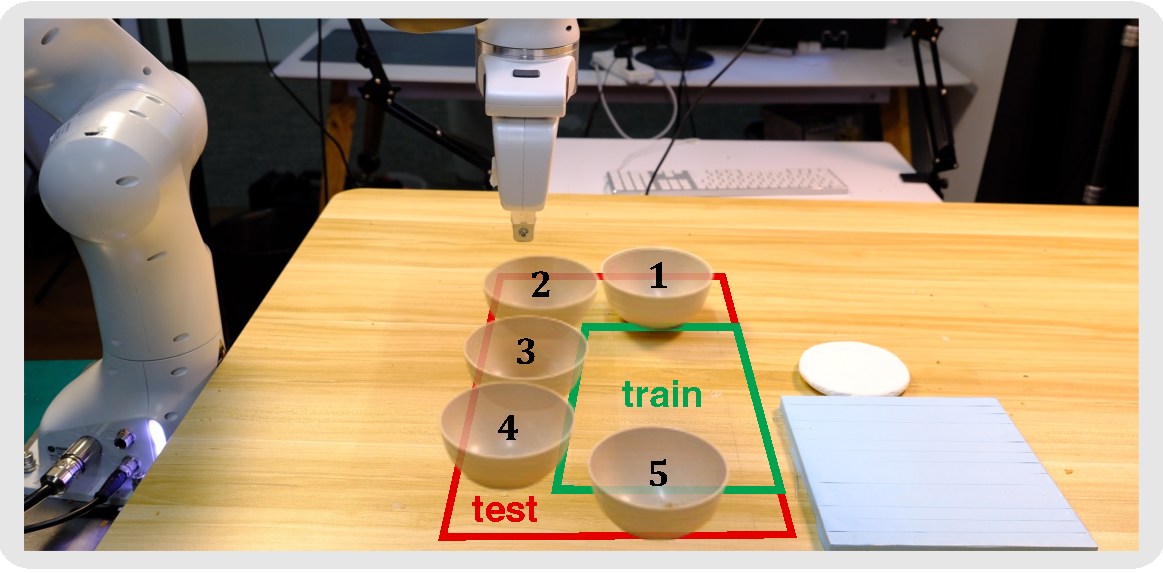
\includegraphics[width=0.40\textwidth]{figures/spatial_generalization.pdf}
\resizebox{0.4\textwidth}{!}{%
\vspace{0.2in}
\begin{tabular}{l|cccccc|ccc}
\toprule


  Spatial Generalization &  1 & 2 & 3 & 4 & 5\\

\midrule
Diffusion Policy & \textcolor{gred}{\XSolidBrush} & \textcolor{gred}{\XSolidBrush} & \textcolor{gred}{\XSolidBrush} & \textcolor{gred}{\XSolidBrush} & \textcolor{gred}{\XSolidBrush} \\
  Diffusion Policy (Depth) & \textcolor{gred}{\XSolidBrush} & \textcolor{gred}{\XSolidBrush} & \textcolor{gred}{\XSolidBrush} & \textcolor{gred}{\XSolidBrush} & \textcolor{gred}{\XSolidBrush} \\
  \textbf{\ours}  & \textcolor{gred}{\XSolidBrush} & \textcolor{ggreen}{\Checkmark} & \textcolor{ggreen}{\Checkmark} & \textcolor{ggreen}{\Checkmark} & \textcolor{ggreen}{\Checkmark} \\
\bottomrule
\end{tabular}}
\vspace{-0.1in}
\end{table}

